\chapter{Architecture}
\label{chapter:architecture}

\section{Introduction}
\label{section:introduction}
In this chapter the implementation tools and the basic architecture are explained. First the used programming language and framework are introduced, then how the different parts of the learning environment work together and finally some frequently used mechanisms are explained.

The source code, tests, this report and all other used scripts and documents can be found on the ETH GitLab at \url{https://gitlab.ethz.ch/flbuetle/bsc-thesis}.

\section{TypeScript}
\label{section:typescript}
JavaScript had its publication in 1996, it is a scripting language and is intended to be used in browsers to extend the possibilities of HTML and CSS. It can dynamically manipulate HTML and CSS, validate user data, send and receive data without reloading the page and much more.
TypeScript extends JavaScript by adding types and can be used anywhere JavaScript runs, because TypeScript code is transformed to JavaScript code by the TypeScript compiler. It provides a way to describe what type a variable has and helps to catch errors before the code is run. Moreover, TypeScript adds, among others, the concepts of method signatures, type interference, interfaces, enumerations and tuples \cite{Typescript}.

\section{Vue.js}
\label{section:vuejs}
Vue.js is a web framework developed by Evan You and its community and was first published in 2014. It is an alternative to Angular and React and was supposed to be a lightweight version of Angular. Vue.js is also based on reusable components, each having its own HTML, JavaScript and CSS.
At the point the development of this project started, Vue.js version 3 was already published. However, Vue.js version 2 is used in this project, because the ecosystem has no caught up yet and many libraries only work with version 2 at the moment \cite{Vue}.

\subsection{Components}
Components are named reusable Vue.js instances and have the advantages that the structure, functionality and style of an element is implemented once and can then easily be used multiple times. Therefore each component has a parent (except from the root component) and possibly multiple child components forming a tree structure \cite{Vue}. 

\subsection{Communication between Components}
Communication between a parent and a child component happens from the parent to the child by properties and from child to parent by events. Properties are custom attributes that pass data from the parent to the child component. Events are emitted by a child component, can carry data and a parent can listen and react upon receiving an event from a child component \cite{Vue}.

\subsection{Best Practices}
The following list represent the best practice that were following in this project. To see examples for each best practice visit the Vue.js style guide  \cite{VueStyleGuide}.

\begin{itemize}
    \item Properties should be as detailed as possible and at least have a type.
    \item Always use \code{key} with \code{v-for} to maintain the internal component state.
    \item Avoid \code{v-if} with \code{v-for}
    \item Only the top-level \code{App} component and layout components should have global styles. All other components should always have scoped styles i.e the styles is only used within the component.
    \item Each component is in its own file.
    \item Filenames are in PascalCase.
    \item Components without any content should be self-closing e.g \code{<Component />} instead of \code{<Component><Component/>}.
    \item Components name casing in templates is PascalCase.
    \item Properties name casing is camelCase.
    \item Elements with multiple attributes should span multiple lines, with one attribute on each line.
    \item Component templates should only contain simple expressions. Complex expressions should be moved into computed properties or methods.
    \item Element attribute values should be quoted.
    \item Directive short hands are always used.
    \item Element attributes should be ordered consistently.
    \item Components should be ordered like \code{<templates>}, \code{<script>} and \code{<style>}.
    \item Element selectors should be avoided with \code{scoped}
    \item Properties and events should be used for parent-child communication.
\end{itemize}

\section{Structure}
\label{section:structure}
The code for the project is located in the \textbf{src} folder. The \textbf{src} folder has the following content: 

\begin{itemize}
    \item \textbf{assets} - all the media i.e images and videos used in the components
    \item \textbf{components} - all components of the project that are not a view
    \item \textbf{router} - everything in Vue.js is a component, but not everything is page. A page needs a route e.g. \code{/settings} and this folder contains all routes of the project. Components with a route are called \textbf{routed}
    \item \textbf{views} - all routed components
\end{itemize}

The \textbf{components} folder is structured as follows:

\begin{itemize}
    \item \textbf{ciphertexts} - all components for \nameref{chapter:keepingInformationSecret}
    \item \textbf{layout} - all components for the layout i.e header and footer
    \item \textbf{numbersystems} - all components for \nameref{section:numberSystems}
    \item \textbf{shared} - all shared components as explained in \nameref{subsection:generalPuprposeComponents}
    \item \textbf{trees} - all components for \nameref{chapter:learningFromData}
    \item \textbf{words} - all components for \nameref{section:similarWords}
\end{itemize}

The \textbf{tests} contains unit, snapshot and end-to-end tests for the project (chapter \ref{chapter:testingAndCI}). The \textbf{tests} contains the following:

\begin{itemize}
    \item \textbf{unit} - all unit and snapshot tests
    \item \textbf{e2e} - all end-to-end tests
\end{itemize}

\section{Basic functionality}
\label{section:basicFunctionality}

\subsection{Home Screen}
The home screen is a view and is the first page seen when visiting the learning environment (figure \ref{fig:homepage}). It has a simple structure: For each available exercise there is a card with an image to illustrate the exercise and its title. The basic ideas for the images are taken from the text book, but most of the time needed some simple photoshopping to make it represent the task reasonably.

\begin{figure} 
    \centering
    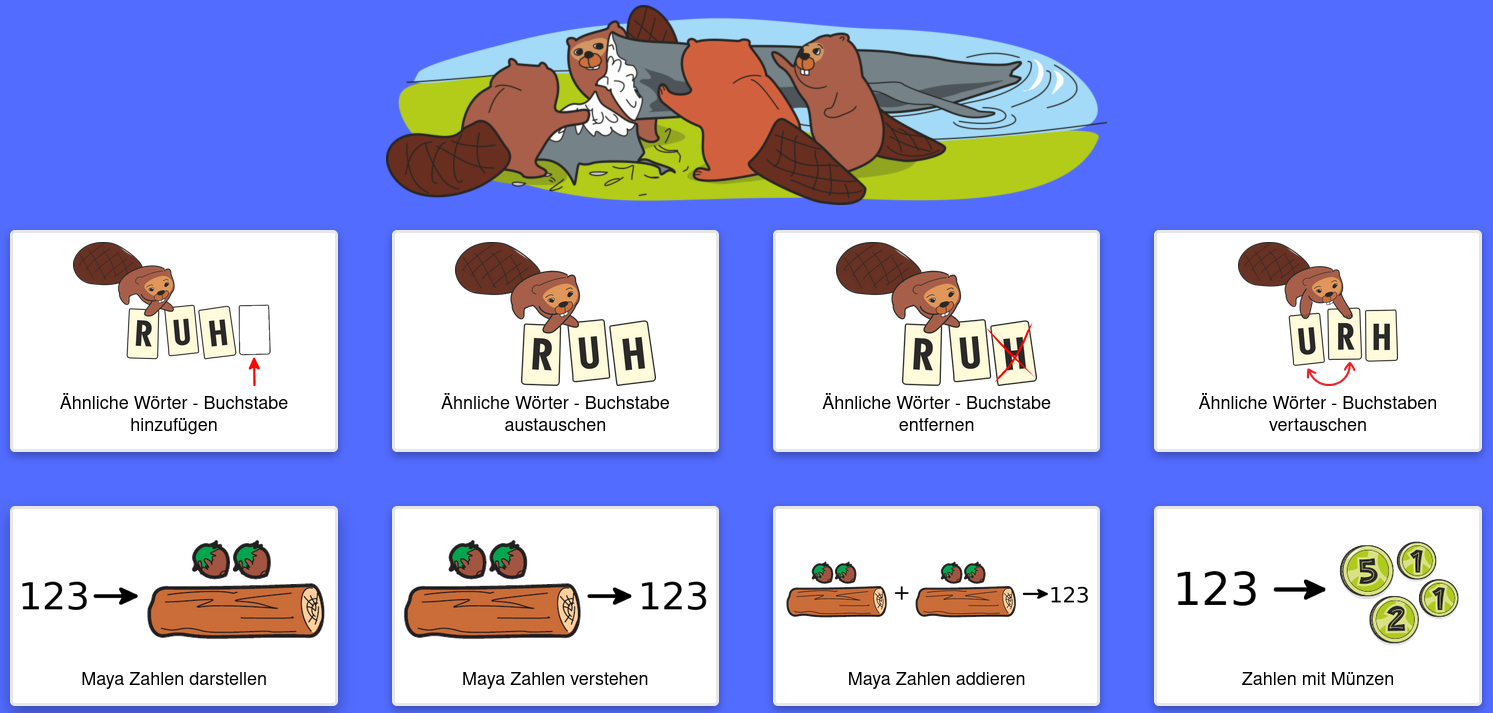
\includegraphics[width=1.0 \columnwidth]{figures/homepage.png}
    \caption{Homepage excerp} 
    \label{fig:homepage} 
\end{figure}

\subsection{Game Mixin and Game Interface}

\subsection*{Game Mixin}
Mixins can be used to reuse functionality over different Vue components. When a component uses a mixin, all functionalities of the mixins are mixed into the component. All exercises use the \code{GameMixin} containing mostly the functionality on starting and evaluating an exercise. Additionally, a function to generate a random number exists to mock random number generation in tests. More on that later.

\subsection*{Game Interface}
Each exercises implements the GameInterface. This ensures that exercise specific functionality like starting and evaluating the exercise is implemented and can be used in the \code{GameMixin}.

%TC:ignore
\begin{lstlisting}[language=TypeScript,caption={GameInterface},label={lst:gameInterface}]
interface GameInterface {
    isInitialized(): boolean;
    start(): void;
    isCorrect(): boolean;
}
\end{lstlisting}
%TC:endignore

\subsection{General Purpose Components}
\label{subsection:generalPuprposeComponents}
The following presented components are components that are crucial or heavily reused. Most of them are part of the user interaction system since all exercises need some kind of user interaction elements.
\TODO{maybe elaborate on technical details like passing events}

\subsection*{Game}
The Game component is the crux of the matter
\TODO{explain game component}

\subsection{Event Bus}
Sometimes components are not in a direct parent-child relationship and still need to communicate. This can still be achieved by passing properties and emitting events, but evolves quickly into an unclear structure. To tackle this problem one can use an event bus. 
The event bus is a vue instance that allows to to emit an event in one component and listen for that event on another component. To use the event bus, a component simply needs to import the instance and can emit or listen for event on the usual way. The event bus is used between the \nameref{subsection:gameButtons} and each exercise.

\subsection*{Game Buttons}
\label{subsection:gameButtons}
Every exercise needs a \textbf{check exercise} and a \textbf{next exercise} button (figure \ref{fig:gameButtons}) to first check a given solution to an exercise and let the system check it and second to load the next exercise.

\begin{figure} 
    \centering
    
\includegraphics[width=0.6 \columnwidth]{figures/game_buttons.png}
    \caption{Game Buttons} 
    \label{fig:gameButtons} 
\end{figure}

\subsection*{Undo}
The Undo button simply restores the current exercise initial conditions, so one can retry it again.

\begin{figure} 
    \centering
    
\includegraphics[width=0.1 \columnwidth]{figures/undo.png}
    \caption{Undo} 
    \label{fig:undo} 
\end{figure}

\subsection*{Trashcan}
The Trashcan (figure \ref{fig:trashcan}) is an area where elements can be dropped to remove them. For example when pupils are asked to remove a letter from a word, they can either drag the letter to this area and drop it or first click on the letter and then on the trashcan to remove it.

\begin{figure} 
    \centering
    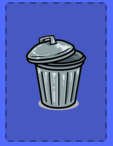
\includegraphics[width=0.1 \columnwidth]{figures/trashcan.png}
    \caption{Trashcan} 
    \label{fig:trashcan} 
\end{figure}

\subsection*{Difficulty Levels}
Some exercises have multiple difficulty levels (figure \ref{fig:difficultyLevels}). For those exercise the Difficulty component is used to change the difficulty level. This component gives the possibility to choose from up to three different difficulty levels indicated by an increasing amount of beavers on the button and a title that is showed on hover.

\begin{figure} 
    \centering
    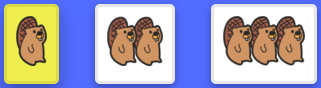
\includegraphics[width=0.4 \columnwidth]{figures/difficulty_level.png}
    \caption{Difficulty levels from easy to hard} 
    \label{fig:difficultyLevels} 
\end{figure}

\subsection*{Tutorial}
To introduce an exercise to the pupils the title of the exercise and a short instruction is not enough. Therefore for each exercise there is a detailed explanation of the background and purpose and a tutorial video (figure \ref{fig:tutorialButton} and figure \ref{fig:tutorialExample}). The tutorial video shows an example run of first giving a wrong solution, restarting the exercise and finally giving the correct solution.
The tutorial videos were recorded by a screen capture tool and the mouse movement on how to solve the exercise is done programmatically. The reason for this is that moving the mouse by hand to solve the exercise introduces a jitter to the mouse movement and might be irritating. The tutorial on the other hand should show clearly and without any hesitation the way on how to solve the exercise. Since this cannot be done by an average human being, the mouse movement is done programmatically. Each graphical element part of the exercise has an ID and one can give a list of IDs that should be visited in a run. The tutorial video then shows a mouse visiting and interacting with these graphical elements and demonstrates how to solve the exercise. 

\begin{figure} 
    \centering
    
\includegraphics[width=0.1 \columnwidth]{figures/tutorial_button.png}
    \caption{Tutorial Button} 
    \label{fig:tutorialButton} 
\end{figure}

\begin{figure} 
    \centering
    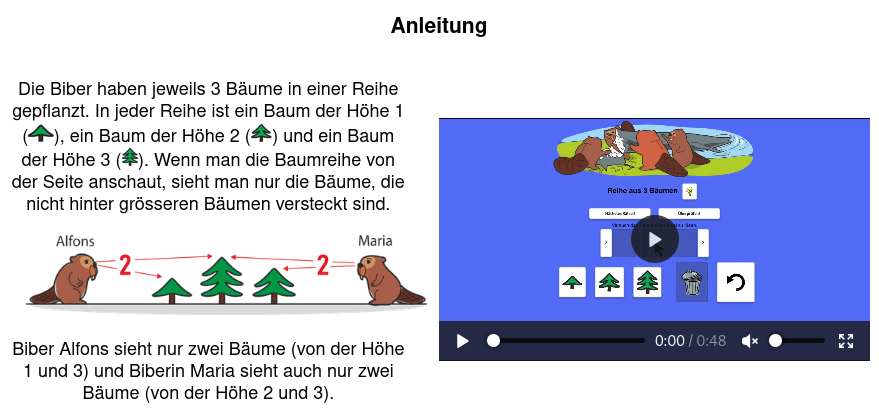
\includegraphics[width=1.0 \columnwidth]{figures/tutorial_example.png}
    \caption{Tutorial of the Row of Trees Exercise} 
    \label{fig:tutorialExample} 
\end{figure}
